\chapter{Domain and Segment Setup} \label{chap:domainsetup}
This chapter explains how a {\ViennaGrid} domain can be filled with cells. Since this
is a necessary step in order to do anything useful with {\ViennaGrid}, it is explained in detail in the following.
Existing file readers and writers are explained in Chapter \ref{chap:io}.

\TIP{A tutorial code can be found in \texttt{examples/tutorial/domain\_setup.cpp}.}

In the following, the simple triangular mesh shown in Fig.~\ref{fig:sampledomain} will be set up.
Thus, the domain type using the provided configuration class for two-dimensional triangular classes will be used:
\begin{lstlisting}
 typedef viennagrid::config::triangular_2d                  ConfigType;
 typedef viennagrid::result_of::domain<ConfigType>::type    DomainType;

 DomainType domain;    //The domain to be set up in the following
\end{lstlisting}
If these lines are used inside a template class or template function, an additional \lstinline|typename| needs to be put after \lstinline|typedef| in the second line.
The created domain object will be filled with vertices and cells in the following.

\begin{figure}[tb]
\centering
 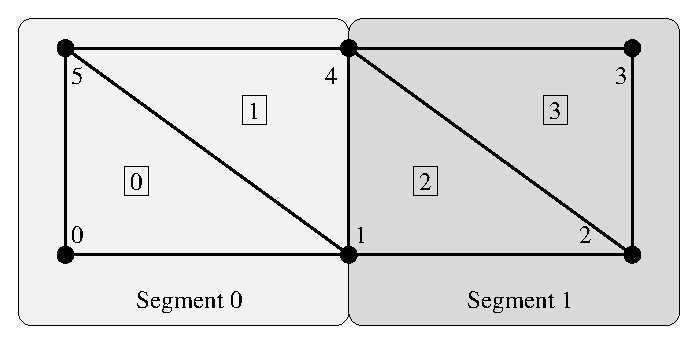
\includegraphics[width=0.65\textwidth]{figures/sampledomain.eps}
 \caption{An exemplary mesh for demonstrating the use of {\ViennaGrid}. Cell-indices are boxed.}
 \label{fig:sampledomain}
\end{figure}


\section{Adding Vertices to a Domain}
Since vertices carry geometric information by means of an associated point type,
we first obtain the respective point type from the meta-function \lstinline|point<>|:
\begin{lstlisting}
 typedef viennagrid::result_of::point<ConfigType>::type    PointType;
\end{lstlisting}
This already allows us to add the vertices shown in Fig.~\ref{fig:sampledomain} one after another to the domain. One example to add the first vertex is to push the respective point to the domain:
\begin{lstlisting}
 PointType p(0,0);
 domain.push_back(p);  // add vertex #0
\end{lstlisting}
The member function \lstinline|push_back| appends the vertex to the domain and assigns the respective ID, provided that the use of IDs is not disabled, cf.~Sec.~\ref{subsec:ncell-ids}.

To push the next vertex, one can either reuse the existing vertex:
\begin{lstlisting}
 p[0] = 1.0;
 p[1] = 0.0;
 domain.push_back(p);  // add vertex #1
\end{lstlisting}
or directly construct the respective points in-place:
\begin{lstlisting}
 domain.push_back(PointType(2,0));  // add vertex #2
 domain.push_back(PointType(2,1));  // add vertex #3
 domain.push_back(PointType(1,1));  // add vertex #4
 domain.push_back(PointType(0,1));  // add vertex #5
\end{lstlisting}
Note that in {\ViennaGridversion} vertices have to be provided in ascending order to the domain. 

\NOTE{In {\ViennaGridversion} vertices always have to be added to the domain directly and cannot be added indirectly via a segment.}

If the geometric location of a particular vertex needs to be adjusted at some later stage, the free function \lstinline|ncells| can be used. To e.g.~access vertex \lstinline|#4|,
\begin{lstlisting}
 viennagrid::ncells<0>(domain)[4]
\end{lstlisting}
returns a reference to the respective element, which can then be manipulated accordingly. 

\TIP{More details on the \lstinline|ncells|-function can be found in Chap.~\ref{chap:iterators} as well as in the reference documentation located in \texttt{doc/doxygen}.}

\section{Adding Cells to a Domain or Segment}
The type of cells in a domain is obtained by the \lstinline|ncell| meta-function. Since triangles are topologically two-dimensional,
one can directly use
\begin{lstlisting}
 typedef viennagrid::result_of::ncell<ConfigType, 2>::type    TriangleType;
\end{lstlisting}
However, it should be emphasized that this type definition does yield the cell type for e.g.~tetrahedral domains.
Thus, the more generic way of defining the cell type is to use the topological dimension stored in the cell tag of the domain configuration class:
\begin{lstlisting}
 typedef ConfigType::cell_tag                                  CellTag;
 typedef viennagrid::result_of::ncell<ConfigType,
                                       CellTag::dim>::type     CellType;
\end{lstlisting}
These two lines reliable return the cell type for all types of domains. Note that an additional \lstinline|typename| is required if these lines are put inside a template class or template function.

For what follows, the vertex type is also required and readily obtained using
\begin{lstlisting}
 typedef viennagrid::result_of::ncell<ConfigType, 0>::type     VertexType;
\end{lstlisting}

An overview of the generic procedure for adding a cell to a domain or segment is the following:
  \begin{itemize}
   \item Set up an array holding the pointers the the vertices \emph{in the domain}. Do not use pointers to vertices defined outside the domain.
   \item Instantiate a cell object and add the array of vertex pointers to the cell
   \item Add the cell to the domain. It will be copied to the domain and can be reused for specifying the next cell.
  \end{itemize}
Thus, the array of vertices is created as usual:
\begin{lstlisting}
 VertexType * cell_vertices[3];
\end{lstlisting}
Instead of hard-coding the number of vertices for a triangle, one can instead use 
\begin{lstlisting}
VertexType * cell_vertices[viennagrid::topology::bndcells<CellTag,0>::num];
\end{lstlisting}
Next, the vertex addresses for the first triangle are stored:
\begin{lstlisting}
 cell_vertices[0] = &(viennagrid::ncells<0>(domain)[0]); // vertex #0
 cell_vertices[1] = &(viennagrid::ncells<0>(domain)[1]); // vertex #1
 cell_vertices[2] = &(viennagrid::ncells<0>(domain)[5]); // vertex #5
\end{lstlisting}

\NOTE{Make sure that the correct cell orientation is used, cf.~Appendix!}

Then, a cell is instantiated and the vertices are set:
\begin{lstlisting}
 CellType cell;
 cell.vertices(cell_vertices); //set cell vertices from above
\end{lstlisting}
Now, the cell is ready to be pushed either to a segment or a domain. 

The example mesh consists of two segments, which have to be created first:
\begin{lstlisting}
 domain.segments().resize(2);
\end{lstlisting}
For completeness it should be mentioned that the segment type can be obtained similar to the domain type from a meta-function:
\begin{lstlisting}
 typedef viennagrid::result_of::segment<ConfigType>::type   SegmentType;
\end{lstlisting}
Two shortcut references to the two segments can be obtained as
\begin{lstlisting}
 SegmentType & seg0 = domain.segments()[0];
 SegmentType & seg1 = domain.segments()[1];
\end{lstlisting}
The cell set up above is then pushed to \lstinline|seg0| as
\begin{lstlisting}
 seg0.push_back(cell);
\end{lstlisting}
As for vertices, cells have to be pushed in ascending order in order to get the correct IDs assigned. Note that the cell is always stored inside the domain - a segment keeps a reference to the cell as well as its boundary cells only.

In the same way the other triangles are pushed to the respective segment. For triangle \lstinline|#3|, the code is
\begin{lstlisting}
 cell_vertices[0] = &(viennagrid::ncells<0>(domain)[2]); // vertex #2
 cell_vertices[1] = &(viennagrid::ncells<0>(domain)[3]); // vertex #3
 cell_vertices[2] = &(viennagrid::ncells<0>(domain)[4]); // vertex #4
 cell.vertices(cell_vertices); //set new cell vertices.
 seg1.push_back(cell);
\end{lstlisting}
It should be noted again that one may also \lstinline|push_back()| the cells directly to the \lstinline|domain| if no segments are used.

\TIP{The restriction of filling segments already at domain setup will be relaxed or removed in future versions of {\ViennaGrid}.}